\documentclass[10pt]{article}
\usepackage[english]{babel}
\usepackage[letterpaper,top=2cm,bottom=2cm,left=3cm,right=3cm]{geometry}
\usepackage{helvet}\renewcommand{\familydefault}{\sfdefault}
\usepackage{setspace,amsmath,amssymb,graphicx,booktabs,longtable,array,float,hyperref}
\setstretch{1.0}\pagestyle{empty}
\graphicspath{{fig/}}
\renewcommand{\thefigure}{S\arabic{figure}}\renewcommand{\thetable}{S\arabic{table}}\renewcommand*{\thesection}{S\arabic{section}}
\newcolumntype{L}[1]{>{\raggedright\arraybackslash}p{#1}}
\title{Supplementary Information for\\ ``TPSGen: an integrated framework for motif-conditioned generation and tissue-bias prioritization of tomato promoters''}
\author{Zhoujie Fan, Xiaoyu Wang, Haimeng Zhang, Hao Meng, Hong Liang, Tong Zhang, \\
Huazhu Fu, Ching-Yu Cheng, Weihua Pan, Xiaohui Yao*, Cheng Zhao*, Shan Cong*}

\date{}
\begin{document}\maketitle
\section{Data Sources and Evaluation Design}
This Supplementary Information describes the datasets, model-development experiments and computational evaluations underlying TPSGen, together with the released software workflow and its reproducible execution routes. The reported numerical results constitute the computational evidence used in this study. They should not be interpreted as wet-lab measurements of promoter activity or tissue specificity.


\subsection{Tomato promoter definition and sequence extraction}
Tomato promoter sequences were derived from the ITAG3.2 genome assembly and GFF3 gene annotation distributed through Phytozome \cite{Goodstein2012,Sato2012}. The annotation contains genomic coordinates, strand assignments and stable gene identifiers used to link promoter sequences with transcript abundance measurements. The original dataset-construction workflow retained records annotated as genes on the positive strand and extracted the 165 nucleotides immediately upstream of each annotated gene start, corresponding to the half-open genomic interval \([\texttt{gene\_start}-165,\texttt{gene\_start})\). For example, a gene starting at position 16,480 contributed the interval \([16{,}315,16{,}480)\). Sequences containing unresolved bases or shorter than 165 bp were excluded.

ITAG3.2 provides gene boundaries rather than experimentally resolved transcription start sites (TSSs) for every gene. Accordingly, gene start was used as a coordinate proxy for TSS-centered extraction. The 165-bp interval was selected as the fixed input length for the promoter-generation and tissue-scoring models, balancing promoter-proximal sequence coverage against model complexity; it should not be interpreted as a universal biological promoter boundary. The model-development dataset used positive-strand genes to maintain a common orientation. When users prepare negative-strand genes for the released tool, the corresponding downstream genomic interval must be reverse-complemented so that every FASTA record is represented in the promoter-to-gene orientation. The resulting model input is one or more 165-bp sequences containing only A, C, G and T.

\subsection{Tomato expression-associated dataset}
Expression measurements were obtained from the MicroTom metabolic network (MMN), a transcriptome and metabolome resource covering tomato organs and developmental stages \cite{Li2020}. The source resource contains measurements from 20 organ--stage conditions, including root, stem, leaf, floral tissues and successive fruit-development stages. The project did not use all of these conditions as model targets. Instead, it selected four measurements intended to represent mature vegetative tissues and mature fruit: root at 85 days post germination (R85), stem at 85 days (S85), leaf at 85 days (L85) and fruit at 15 days after breaker stage (Br15). In the remainder of this supplement, ``root'', ``stem'', ``leaf'' and ``fruit'' refer to these four project-defined measurements.

The promoter table and the MMN expression table were joined by their shared gene identifiers. Records without a valid promoter sequence or a matching expression record were excluded. The four selected expression columns were then transformed with \(\log(1+x)\) to reduce the dynamic range while retaining zero-valued measurements. After transformation, values below 0.01 were set to zero and the remaining values were rounded to three decimal places. The project also removed 2,966 genes whose values were zero in all four selected tissues, because these records provide no tissue-associated signal for supervised learning. The resulting ITAG-MMNP2E resource contained 14,071 promoter--target records, each consisting of one 165-bp sequence and four processed target values. This is the post-matching, post-quality-control total used in the original experiment; the available project description does not provide a complete count for every intermediate exclusion category. The data definitions and their roles are summarized in Table~\ref{tab:data-resources}.

For the TransVAE-MLP model-development experiment, the 14,071 records were randomly divided at the sequence level into 11,257 training, 1,404 validation and 1,407 test records. The validation set was used for model selection and the test set for prediction assessment. This split defines the computational evaluation reported here; it is not an independent external test set or a substitute for biological validation.

\begin{table}[H]
\centering
\caption{Data resources and experimental roles used in the integrated workflow.}
\label{tab:data-resources}
\begin{tabular}{L{0.23\textwidth}L{0.25\textwidth}L{0.38\textwidth}}
\toprule Resource & Verified size or format & Role in this study \\
\midrule
ITAG3.2 genome and annotation & Genome FASTA and GFF3 annotation & Gene coordinates, strand information and promoter-window extraction. \\
MMN transcriptome measurements & 20 organ--stage conditions; four selected project targets & Source of R85, S85, L85 and Br15 expression-associated labels. \\
ITAG-MMNP2E & 14,071 records; 165-bp sequence plus four targets & TransVAE-MLP training, validation and test experiment. \\
DNABERT pretraining set & 34,725 sequences; 500-bp promoter-related input & 6-mer masked-language-model pretraining. \\
DNABERT fine-tuning set & 4,448 balanced 165-bp examples & Promoter/non-promoter classification. \\
preGAN paired set & 5,100 paired records; reported split 3,570/765/765 & Conditional masked-position generation. \\
Fruit-expression predictor resources & DenseNet--LSTM checkpoint and training log are bundled; the original training table is not bundled with a verified provenance record & Frozen scalar-expression constraint used by the preGAN route; not presented as a newly trainable or independently benchmarked dataset. \\
\bottomrule
\end{tabular}
\end{table}

\subsection{DNABERT and preGAN datasets}
The DNABERT pretraining and fine-tuning datasets served different purposes and used different sequence lengths. Self-supervised pretraining used 34,725 500-bp sequences extracted upstream of ITAG3.2 gene starts and an 80:20 training/validation partition. Supervised fine-tuning used 4,448 independent 165-bp examples, comprising equal numbers of promoter sequences and randomly sampled non-promoter genomic segments. These records were divided 70:15:15 into training, validation and test sets. The 500-bp pretraining context must therefore not be confused with the 165-bp sequence accepted by the downstream classification and integrated design workflow.

Two related datasets were used for preGAN. The conditional generator used 5,100 promoters selected for high Br15-associated expression. DNABERT-derived high-evidence positions were retained in \texttt{realA}, while editable positions were replaced by \texttt{M}; the complete reference sequence was stored as \texttt{realB}. The reported paired-set split was 3,570/765/765 (training/validation/test). A separate fruit predictor supplied the scalar generation constraint; its original training table and record-level partition are not included in the release.

\subsection{Evaluation metrics and evidence boundaries}
We used task-specific metrics: PCC for expression-score or k-mer-frequency agreement, accuracy/F1/MCC for promoter classification, perplexity for masked-token prediction, edit distance and BLAST E-values for sequence comparison, and non-masked retention for conditional fidelity. Model scores, motif evidence and tissue-bias statistics are computational outputs; they are not direct measurements of TF binding, promoter activity or tissue specificity in planta.

Tissue-associated bias was summarized with
\[
\tau=\frac{\sum_{i=1}^{n}(1-x_i/x_{\max})}{n-1},
\]
where \(x_i\) is the predicted value for tissue \(i\), \(x_{\max}\) is the maximum value across tissues and \(n=4\). Values approaching one indicate a more concentrated predicted profile, whereas values approaching zero indicate a more even profile. The favored tissue is identified from the largest score, not from \(\tau\) alone.

\section{DNABERT Motif Evidence}
\subsection{6-mer pretraining and promoter classification}
The original tomato promoter experiment followed the DNABERT sequence-language-model formulation \cite{Ji2021}. Each nucleotide sequence was converted to overlapping 6-mers with a one-nucleotide stride. Thus, a 500-bp pretraining sequence and a 165-bp fine-tuning sequence represented different experimental stages rather than interchangeable model inputs. The 500-bp sequences supplied broader promoter-related context during self-supervised pretraining, whereas the 165-bp examples defined the promoter/non-promoter classification task and matched the fixed sequence length subsequently used by the integrated design workflow.

Pretraining used masked-language modeling: 15\% of the token positions were selected for corruption and the model learned to recover the original token from its surrounding sequence context. The original configuration used 200,000 training steps, learning rate \(4\times10^{-4}\), weight decay 0.01, 12 Transformer layers and 12 attention heads. Six-mers were retained because they were the tokenization setting used to train the available project model and are consistent with the published DNABERT formulation; this supplement does not claim that \(k=6\) is universally optimal for tomato promoter analysis. The selected pretraining model reached a reported perplexity of 3.98.

The pretrained encoder was subsequently fine-tuned to distinguish 165-bp promoter sequences from balanced non-promoter genomic segments. Performance was assessed on the held-out portion of the 70:15:15 split described in Section S1.3. The reported test values were Accuracy 0.905, F1 0.906 and MCC 0.813 (Table~\ref{tab:dnabert-results}). These values support the promoter-classification task under the original split; they are not an evaluation of motif binding or candidate promoter activity.

\begin{table}[H]\centering
\caption{Reported DNABERT experiment settings and test results.}\label{tab:dnabert-results}
\begin{tabular}{L{0.38\textwidth}L{0.42\textwidth}}\toprule Item & Reported value \\\midrule
Pretraining input & 34,725 sequences; 500-bp context \\
Fine-tuning input & 4,448 balanced 165-bp examples \\
Objective & 6-mer masked-language modeling; 15\% masking \\
Pretraining result & Perplexity 3.98 \\
Classification result & Accuracy 0.905; F1 0.906; MCC 0.813 \\
\bottomrule\end{tabular}\end{table}

\subsection{Position-wise evidence and motif localization}
The original interpretation workflow extracted token-level attention-derived evidence from the fine-tuned classifier and projected it back onto nucleotide coordinates. Because adjacent 6-mers overlap, a nucleotide may be covered by several tokens; position-wise evidence therefore summarizes model evidence associated with overlapping local sequence contexts rather than an independent score for a single base. Promoter and random-gene sequences were processed using the same mapping convention so that their positional profiles could be compared.

The promoter profile showed a concentrated signal approximately 50--30 bp upstream of the project TSS reference, whereas the random-gene profile was more diffuse. This location is reported relative to the coordinate convention used in the original experiment. It should not be interpreted as a universally resolved core-promoter boundary, because gene start served as a TSS proxy and the source annotation did not provide experimentally mapped TSSs for every record. Attention-derived evidence indicates positions used by the classifier, but attention alone does not demonstrate transcription-factor occupancy or causal regulatory activity.

\subsection{Motif summary and in-silico mutagenesis}
High-evidence sequence segments were collected across promoter records and consolidated into recurrent short sequence patterns. The resulting summary included CTATT, ACTAA, ATCCA and TTTAT with 239, 188, 184 and 121 retained instances, respectively. These counts refer to retained model-derived sequence instances, not to numbers of experimentally validated transcription-factor binding sites. The thresholds used for enrichment and similarity merging define model-derived motif evidence rather than experimentally confirmed motif occurrences.

In-silico mutagenesis provided a second computational check on the high-evidence regions. Bases within selected regions were perturbed and the resulting change in masked-language-model loss was compared with the unperturbed sequence. A loss increase indicates that the trained sequence model found the original local context easier to explain than the perturbed context. This supports model-learned sequence constraint, but it does not identify the cognate transcription factor or establish promoter function in vivo.

For each recurrent pattern, the corresponding high-evidence segments were aligned and visualized as sequence logos. The horizontal axis denotes position within the aligned local sequence window, not a genomic or TSS-relative coordinate, and the vertical axis shows nucleotide counts. The logos therefore summarize recurrent local patterns identified by DNABERT rather than experimentally validated binding sites. The corresponding four-panel summary is shown in Fig.~\ref{fig:supp-dnabert}.

\begin{figure}[H]
\centering
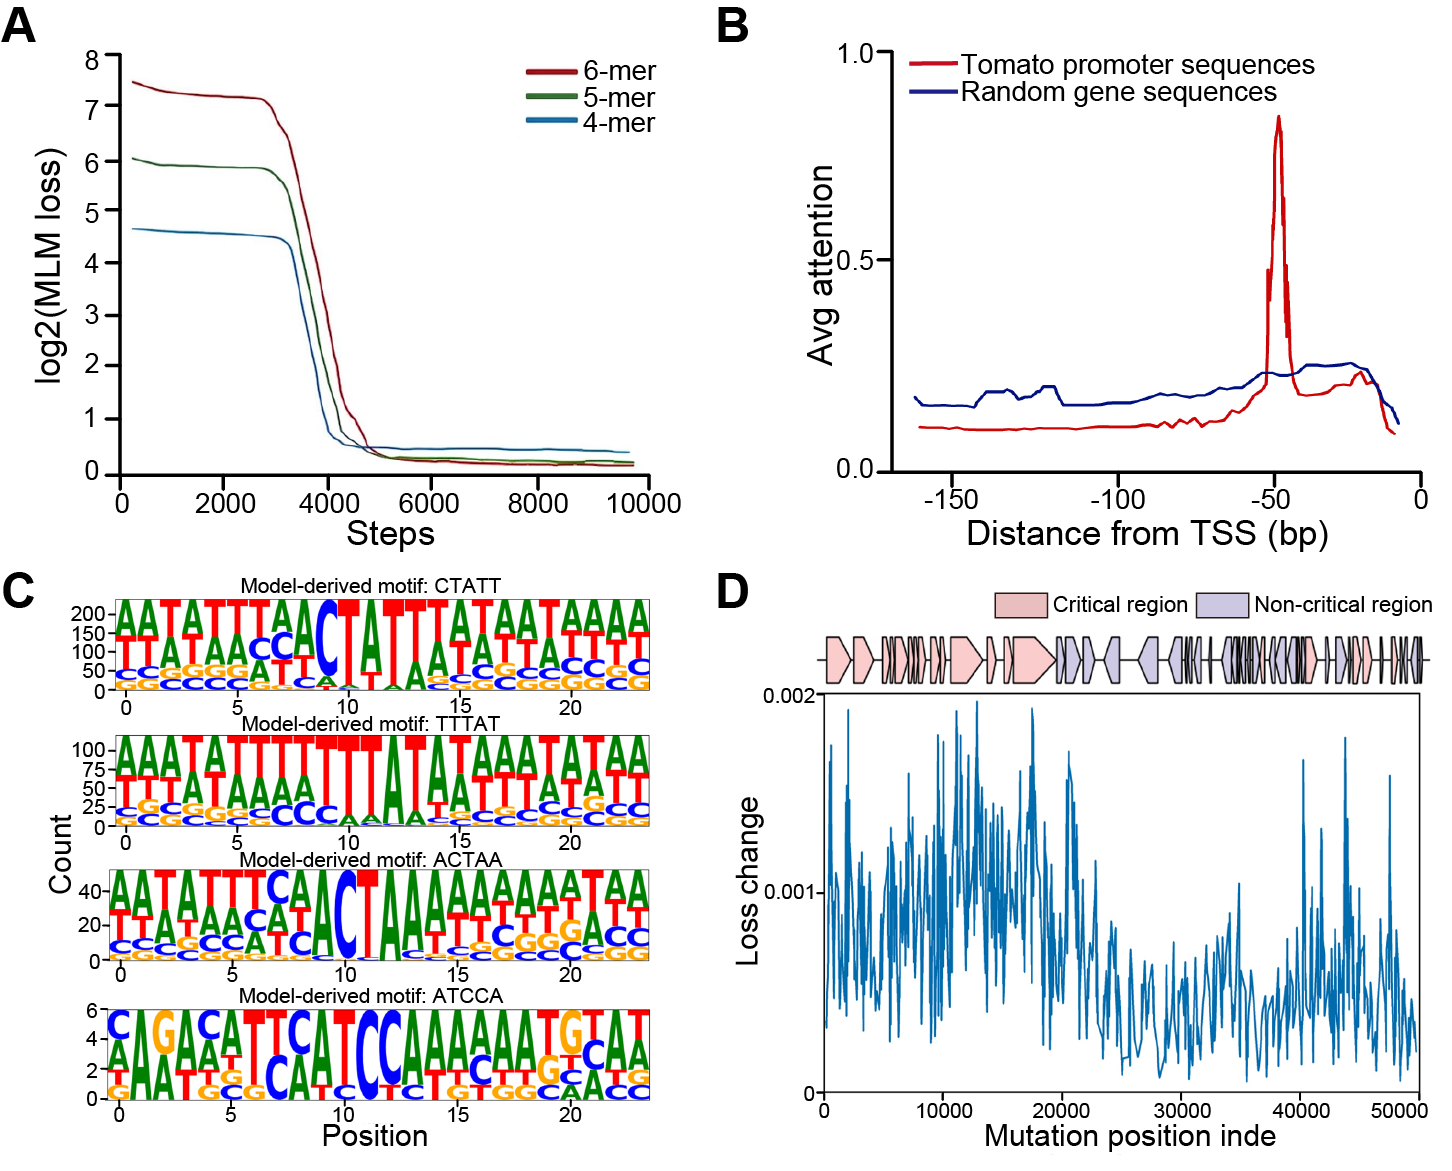
\includegraphics[width=\textwidth]{supp_fig1.png}
\caption{DNABERT pretraining, positional evidence, recurrent motif patterns and in-silico mutagenesis. (A) Masked-language-model pretraining loss for 4-mer, 5-mer and 6-mer tokenization. (B) Average attention-derived evidence across tomato promoter sequences and random gene sequences, shown relative to the project TSS coordinate proxy. (C) Sequence logos for recurrent model-derived patterns identified from high-evidence regions. (D) Retained computational mutagenesis result showing the change in model loss across the mutation index; the upper track indicates the critical and non-critical regions defined in the original analysis. These panels reproduce the DNABERT analyses from the original tomato promoter study. The attention, motif and mutagenesis signals represent model-derived sequence evidence and do not by themselves establish transcription-factor binding or promoter activity.}
\label{fig:supp-dnabert}
\end{figure}

\subsection{Relevance to the released tool}
In TPSGen, the model-backed DNABERT route accepts canonical 165-bp tomato promoter sequences and reports promoter evidence and position-associated evidence when the required fine-tuned model resources are available. These outputs can be used to nominate sequence regions for retention during conditional candidate generation. The package also exposes a deterministic exact-match scanner as a transparent fallback. Exact matches from that scanner are operational motif annotations; they are not equivalent to rerunning the historical attention, enrichment and mutagenesis analyses. Output provenance identifies the backend used so that model-derived evidence and deterministic motif matches are not conflated.

\section{preGAN Motif-Conditioned, Fruit-Guided Generation}
\subsection{Conditional input construction}
The preGAN experiment was designed as conditional sequence completion rather than unconstrained de novo generation. Its paired training set contained 5,100 tomato promoter records selected for high Br15-associated expression, with the 3,570/765/765 split described in Section S1.3. For each complete 165-bp reference sequence, denoted \texttt{realB}, DNABERT-derived high-evidence regions were retained while designated editable positions were replaced by \texttt{M}, producing the corresponding condition sequence \texttt{realA}. The retained positions supplied the sequence context that generation was intended to preserve; the masked positions defined where alternative bases could be generated.

Complete sequences were represented by four-channel nucleotide encodings. In the historical implementation, known bases in \texttt{realA} retained their nucleotide encoding, whereas each \texttt{M} position was initialized by a four-dimensional random vector. The generator converted this mixed condition representation into an \(L\times4\) matrix of nucleotide probabilities, where \(L=165\). A discrete candidate sequence was then obtained from the per-position nucleotide outputs. Because the mask was constructed from upstream DNABERT evidence, the resulting preservation behavior depends on both the DNABERT region-selection procedure and the conditional generator; it should not be generalized to arbitrary experimentally verified motifs.

\subsection{Generator, critic and fruit-guidance predictor}
The original preGAN combined a conditional WGAN-GP generator and critic with a separately pretrained DenseNet--LSTM expression predictor. The generator mapped the condition sequence through a 512-dimensional projection, multi-head attention, five one-dimensional convolutional residual blocks and a final four-channel softmax output. The critic received either the real pair \([\texttt{realA},\texttt{realB}]\) or the generated pair \([\texttt{realA},G(\texttt{realA})]\), concatenated across channels. Conditioning the critic on \texttt{realA} allowed it to assess compatibility with the supplied sequence context in addition to distinguishing generated and reference sequences.

The generator objective combined three terms:
\[
\mathcal{L}_{G}=\mathcal{L}_{\mathrm{adv}}+
\lambda_{L1}\mathcal{L}_{L1}+
\lambda_{\mathrm{pred}}\mathcal{L}_{\mathrm{pred}}.
\]
The adversarial term encouraged candidates to approach the conditional reference-sequence distribution. The \(L1\) term was evaluated at non-masked positions and penalized changes to retained sequence context. The predictor term penalized deviation between the predicted scalar fruit-associated value of \(G(\texttt{realA})\) and the specified target value. Thus, motif conditioning and fruit guidance entered the objective through distinct mechanisms: the conditional template and non-masked consistency term controlled where sequence context was retained, whereas the frozen scalar predictor directed generated candidates toward the fruit-associated target. The predictor did not output a four-tissue profile and did not directly optimize the contrast between fruit and non-fruit tissues. It supplied a computational optimization signal rather than an experimental measurement of promoter activity.

The fruit-expression predictor used convolutional, recurrent and densely connected feature-extraction components followed by a scalar regression output and was optimized with mean-squared error before integration into preGAN. The available predictor checkpoint and training log support the reported model configuration, but the associated training script refers to an external absolute-path CSV that is not included in the release. Consequently, a complete record-level reconstruction of the predictor training partition is not available in the repository. The model-comparison analysis reported a PCC of 0.72 for the DenseNet--LSTM predictor; this value is a computational result for the predictor used in the preGAN design experiment.

Generator and critic learning rates were \(1\times10^{-4}\), the gradient-penalty coefficient was 10, batch size was 32 and training ran for 10,000 iterations. The critic was updated five times per generator update, and intermediate model and sequence outputs were recorded every 100 iterations. These settings describe the preGAN model-development experiment and are not package-wide defaults.

\subsection{Sequence similarity and non-masked retention}
Sequence-distribution learning was monitored by comparing 4-mer frequency vectors from generated and reference promoters at iterations 99, 4,999 and 9,999. The progressively closer profiles were used as a training diagnostic. In the final regional analysis, 4-mer frequencies were calculated over the full 165-bp sequence and over two project-defined terminal windows: the first 20 bp and the last 20 bp in the stored sequence orientation. Generated-versus-reference PCC values were 0.98, 0.77 and 0.86 for the full, first-20-bp and last-20-bp analyses, respectively. These labels describe computational sequence windows; without experimentally resolved TSSs and strand-complete extraction, they should not be treated as universally defined proximal and distal promoter compartments.

A separate model comparison evaluated 4-, 5- and 6-mer frequency agreement. The preGAN analysis yielded PCC values of 0.95, 0.93 and 0.89, compared with 0.92, 0.90 and 0.88 for TransVAE-MLP-generated sequences and 0.91, 0.88 and 0.86 for the comparison WGAN. These aggregate frequency correlations assess similarity of short-word distributions and do not establish that individual candidates are functional promoters.

Conditional fidelity was measured at retained positions. Let $x=\texttt{realB}$, $\hat{x}=G(\texttt{realA})$, and $\Omega_R=\{i:\texttt{realA}_i\neq\texttt{M}\}$. The retention rate was
\[
R_{\mathrm{retain}}=100|\Omega_R|^{-1}
\sum_{i\in\Omega_R}\mathbb{I}(\hat{x}_i=x_i),
\]
where \(\mathbb{I}\) is the indicator function. The reported value was 99.55\%, indicating high sequence agreement at condition-bearing positions; it does not establish that every retained position is a functional motif.

\subsection{Candidate diversity and fruit-associated prioritization}
Pairwise edit-distance distributions were compared among generated, natural and random sequences. BLAST searches against the project tomato sequence database provided a complementary measure of database similarity. The generated-sequence distributions occupied an intermediate range rather than exactly matching the natural or random controls. These analyses were used to detect direct copying and gross departure from tomato-like sequence space; edit distance and BLAST similarity are not measures of transcriptional function or sequence novelty by themselves.

For downstream prioritization, 20 generated candidates were sampled and scored for R85, S85, L85 and Br15 using the TransVAE-MLP scoring model described in Section S4. Eighteen candidates had \(\tau>0.7\), including eight near or above 0.8; the complete range was 0.658--0.879. Their Br15-associated scores were generally higher than the other three scores in this selected visualization. Because both candidate selection and assessment were computational and used project-related models, this analysis demonstrates model-consistent fruit-associated prioritization rather than independent validation of fruit-specific expression.

\begin{figure}[H]
\centering
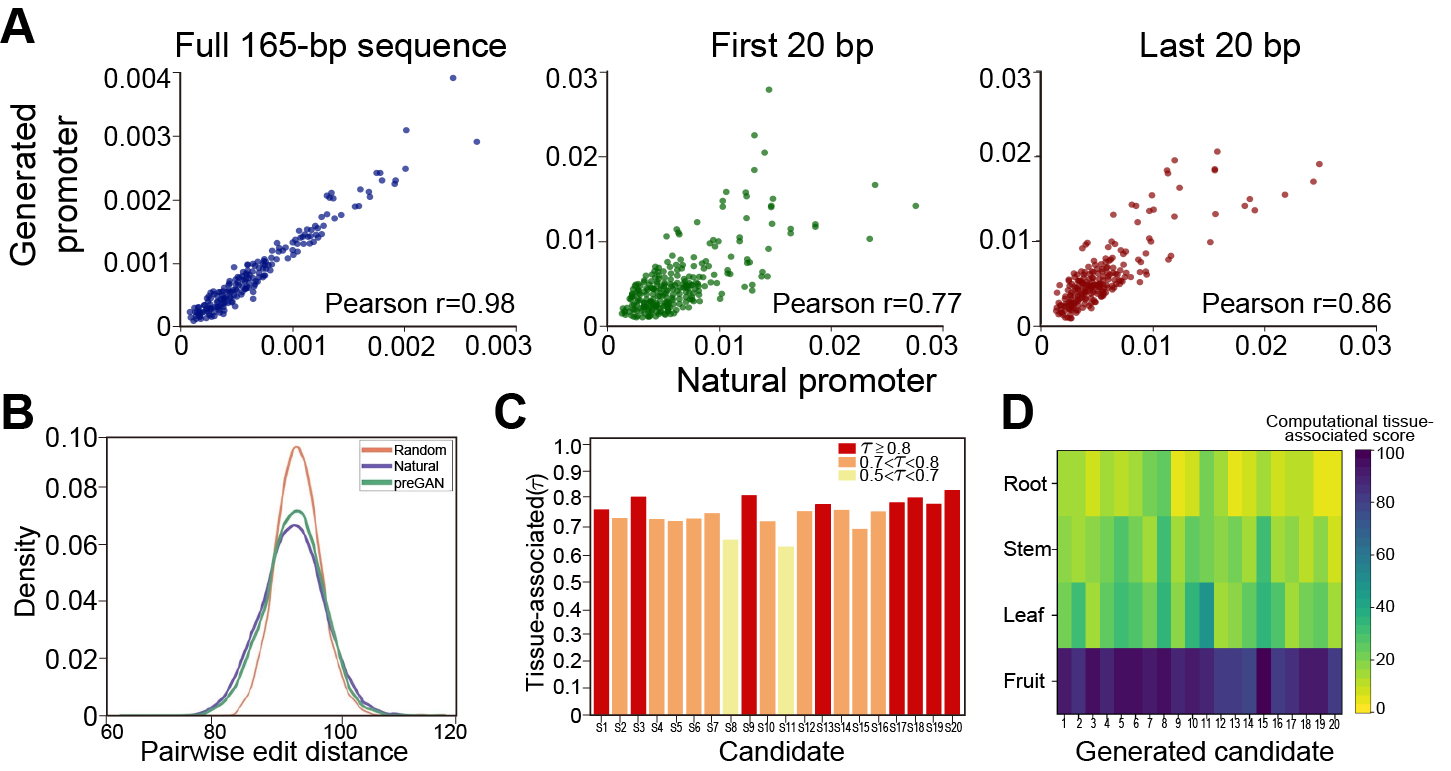
\includegraphics[width=\textwidth]{supp_fig2.png}
\caption{preGAN-generated promoter sequence similarity, diversity and tissue-associated prioritization. (A) Correlation between 4-mer frequency distributions of natural and preGAN-generated promoters for the full 165-bp sequence, the first 20 bp and the last 20 bp. (B) Pairwise edit-distance distributions for random, natural and preGAN-generated sequences. (C) Tissue-associated index \(\tau\) for 20 generated candidates. (D) Computational tissue-associated scores for the same candidates across root, stem, leaf and fruit targets. The candidate scores and \(\tau\) values are computational prioritization outputs rather than experimentally measured expression values.}
\label{fig:supp-pregan}
\end{figure}

\begin{table}[H]\centering
\caption{Reported preGAN generation and computational-prioritization results.}\label{tab:pregan-results}
\begin{tabular}{L{0.46\textwidth}L{0.34\textwidth}}\toprule Evaluation & Reported value \\\midrule
4-mer PCC, full/first 20 bp/last 20 bp & 0.98 / 0.77 / 0.86 \\
4-/5-/6-mer PCC, preGAN & 0.95 / 0.93 / 0.89 \\
Non-masked-position retention & 99.55\% \\
20-sequence tissue analysis & 18 of 20 with \(\tau>0.7\); range 0.658--0.879 \\
\bottomrule\end{tabular}\end{table}

\begin{figure}[H]
\centering
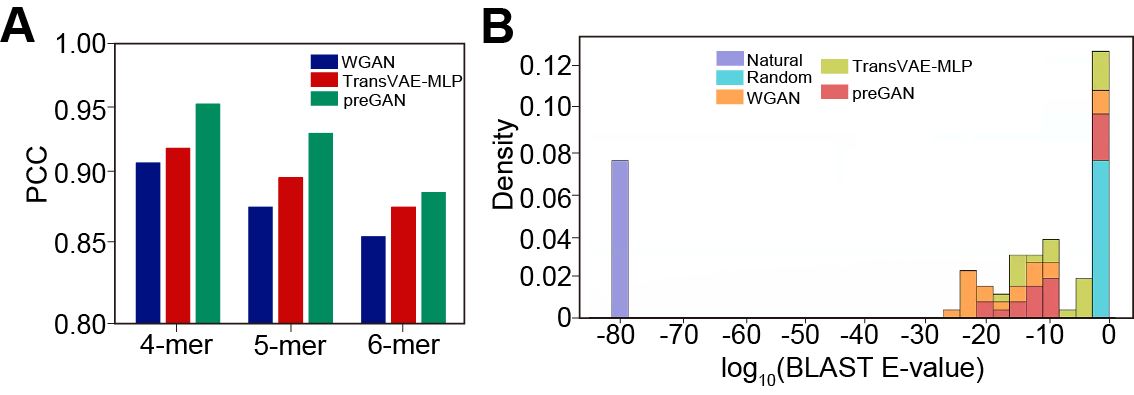
\includegraphics[width=\textwidth]{supp_fig3.png}
\caption{Additional preGAN sequence-distribution and database-similarity comparisons. (A) PCC values between generated and natural promoter k-mer frequency distributions at 4-mer, 5-mer and 6-mer scales for WGAN, TransVAE-MLP and preGAN. (B) BLAST E-value distributions for natural, random, WGAN-generated, TransVAE-MLP-generated and preGAN-generated promoter sequences. These analyses evaluate sequence-distribution similarity and database similarity of the generated candidates; they do not constitute direct measurements of promoter function or tissue-specific activity.}
\label{fig:supp-pregan-comparison}
\end{figure}

\subsection{Relevance to the released tool}
The repository provides the preGAN model components, masked-template data handling, training entry point and checkpoint-backed candidate-generation interface. These components preserve the condition-pair semantics and support software-level execution of the generator and critic. The bundled preGAN generator checkpoint is available for the released route; the quantitative results in Table~\ref{tab:pregan-results} describe the model-development and evaluation experiment. The DenseNet--LSTM resource is an expression-constraint model and is not itself a sequence-generator checkpoint.

Accordingly, the standard installed workflow uses the released package-native candidate generator unless a compatible preGAN generator checkpoint is supplied explicitly. With such a checkpoint, the preGAN workflow accepts one or more 165-bp masked tomato promoter templates, generates the requested number of candidates, and can pass them to the selected scoring backend while recording the design and scoring backends in a provenance manifest. The preGAN evaluation results describe computational sequence generation and prioritization, not experimental validation of promoter function.

\section{TransVAE-MLP Four-Tissue Scoring and Bias Assessment}
\subsection{Scoring mechanism}
The original TransVAE-MLP was trained as a joint sequence-representation, reconstruction and expression-associated regression model. A 165-bp promoter was converted to nucleotide tokens with positional information and passed through a Transformer encoder. The encoder and convolutional bottleneck parameterized the mean and variance of a continuous latent distribution, from which a latent representation \(z\) was obtained by reparameterization. During joint training, the Transformer decoder used this representation for sequence reconstruction, while an MLP mapped the representation to four continuous outputs corresponding, in order, to R85, S85, L85 and Br15.

The historical training objective can be summarized as
\[
\mathcal{L}_{\mathrm{total}}=
\mathcal{L}_{\mathrm{recon}}+
\beta\mathcal{L}_{\mathrm{KL}}+
\lambda_{\mathrm{pred}}\mathcal{L}_{\mathrm{pred}}+
\lambda_{\mathrm{tri}}\mathcal{L}_{\mathrm{3mer}}.
\]
The reconstruction term trained nucleotide recovery, the KL term regularized the latent distribution, the prediction term used the four processed MMN targets and the 3-mer term constrained aggregate local sequence composition. A ten-epoch KL warm-up was used in the original experiment. This joint objective explains why the latent representation can support both reconstruction/generation analyses and tissue-associated scoring, but it does not imply that the four outputs are calibrated measurements of promoter activity.

The original configuration used three Transformer encoder layers, three decoder layers, four attention heads, batch size 128, 300 epochs, learning rate 0.0002 and weight decay 0.05. In the released scoring route, only the encoder-side representation and MLP head are required. The deterministic mean of the encoded latent distribution is used to produce one four-value score vector for each input sequence; stochastic decoding is not part of the released scoring command.

\subsection{Prediction performance}
Prediction performance was evaluated on the held-out test portion of the 14,071-record ITAG-MMNP2E experiment described in Section S1.2. For each target column, PCC was calculated between the predicted and processed reference values across test records. TransVAE-MLP reached PCC values of 0.77, 0.82, 0.79 and 0.78 for R85, S85, L85 and Br15, respectively. These correlations evaluate ranking agreement under the original sequence-level split. They do not measure absolute calibration, transfer to another tomato annotation release or generalization to experimentally synthesized candidates.

The thesis also compared several prediction architectures on the same project dataset. The pure Transformer comparator reported 0.81, 0.85, 0.78 and 0.82, whereas TransVAE-MLP reported the values above. This comparison indicates that TransVAE-MLP was not uniformly the strongest standalone regressor; its project role combined latent sequence modeling with four-target scoring. The Application Note therefore uses the model as a retained scoring component and does not claim a new state-of-the-art expression predictor.

\subsection{Candidate score profiles and tissue-bias prioritization}
The historical TransVAE design experiment searched its learned latent space and decoded selected latent representations into candidate promoter sequences. Twenty generated candidates were sampled for presentation and scored across the four project targets. Four had \(\tau>0.7\), 14 had \(0.5<\tau<0.7\), and two had \(0.4<\tau<0.5\). The associated candidate-by-target heatmap indicated that many displayed candidates had higher Br15-associated scores than their other three scores. Because the same project model family contributed to candidate generation and assessment, this was an internal computational characterization rather than an independent validation experiment.

For current package outputs, tissue bias is assessed from the complete four-value score profile rather than from the target score alone. For a requested target tissue, denoted by \(t\), TPSGen reports the target score \(s_t\) and the target-bias margin
\[
\Delta_t=s_t-\max_{j\ne t}s_j,
\]
and \(\tau\). A positive \(\Delta_t\) indicates that the requested target has the highest score, while its magnitude measures separation from the strongest non-target output. The \(\tau\) statistic describes how concentrated the four-score profile is but does not identify the favored tissue by itself; it must therefore be interpreted together with the preferred target and \(\Delta_t\). These quantities support within-checkpoint candidate ranking. Their numerical scale is checkpoint-specific, and they should not be interpreted as TPM values, experimental fold changes or direct evidence of tissue specificity in planta.

\begin{figure}[H]
\centering
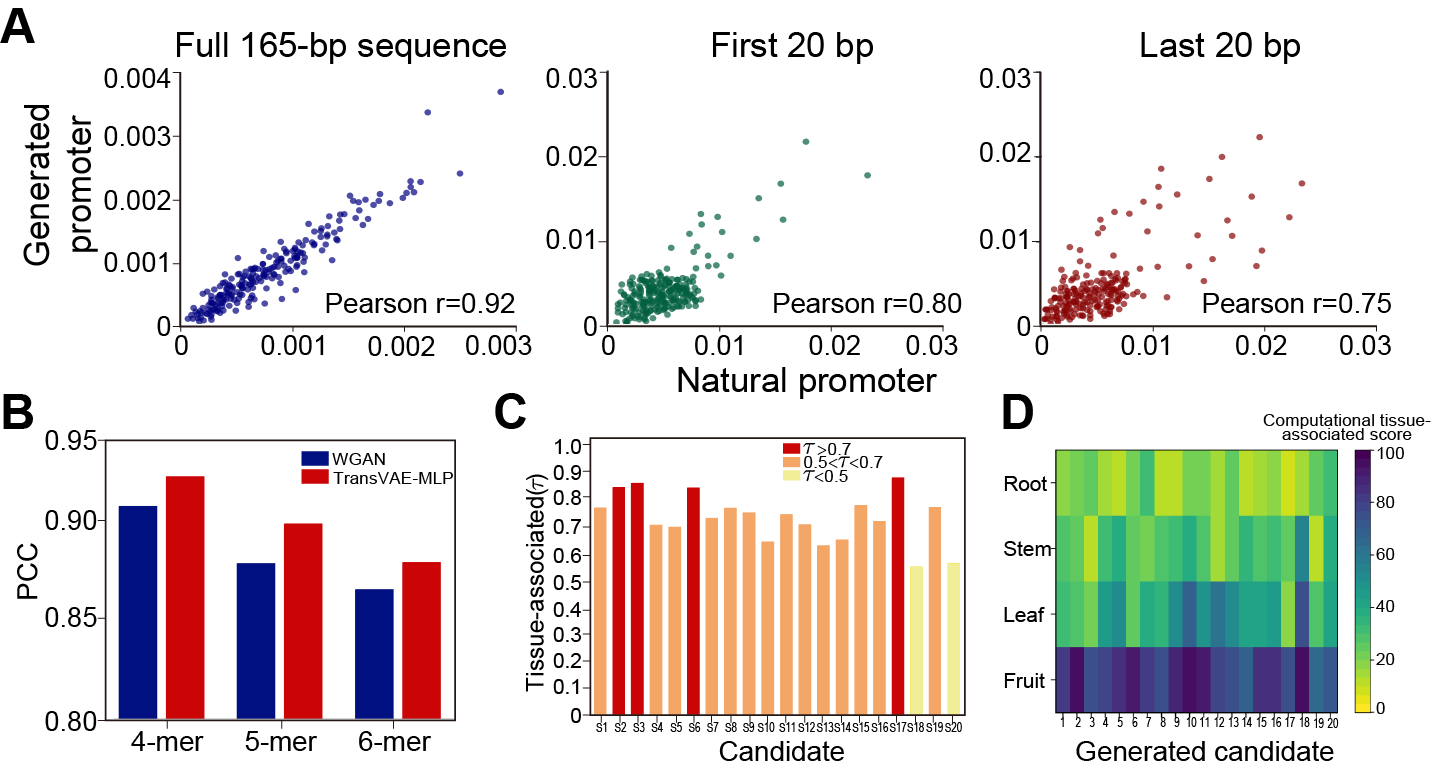
\includegraphics[width=\textwidth]{supp_fig4.png}
\caption{TransVAE-MLP sequence-generation and tissue-associated scoring results. (A) Correlation between natural and TransVAE-MLP-generated 4-mer frequency distributions for the full 165-bp sequence, the first 20 bp and the last 20 bp. (B) PCC comparison between WGAN- and TransVAE-MLP-generated sequences across 4-mer, 5-mer and 6-mer frequency distributions. (C) Tissue-associated index \(\tau\) for 20 TransVAE-MLP-generated candidates. (D) Computational TransVAE-MLP scores for root, stem, leaf and fruit across the same candidates. Scores are model outputs on the project-defined targets and should not be interpreted as experimentally measured expression values.}
\label{fig:supp-transvae}
\end{figure}

\begin{table}[H]\centering
\caption{Reported TransVAE-MLP experiment settings and scoring results.}\label{tab:transvae-results}
\begin{tabular}{L{0.46\textwidth}L{0.34\textwidth}}\toprule Item & Reported value \\\midrule
Training/validation/test records & 11,257 / 1,404 / 1,407 \\
Encoder/decoder layers; attention heads & 3/3; 4 heads \\
Batch size; epochs; learning rate & 128; 300; 0.0002 \\
PCC for R85/S85/L85/Br15 & 0.77 / 0.82 / 0.79 / 0.78 \\
20-sequence \(\tau\) summary & 4 above 0.7; 14 at 0.5--0.7; 2 at 0.4--0.5 \\
\bottomrule\end{tabular}\end{table}

\subsection{Relevance to the released tool}
TPSGen distributes the compatible TransVAE-MLP architecture and a tomato checkpoint for four-target inference. The model-backed scoring route accepts one or more canonical 165-bp A/C/G/T sequences and writes the four scores, preferred target and checkpoint provenance. The integrated workflow applies the same scorer to original and generated candidates so that ranking is performed on a common checkpoint-specific scale.

The repository retains training code to document the model skeleton and data interface, but users do not need to retrain the model for standard scoring. Conversely, the historical latent-space genetic-algorithm design procedure is not exposed as a validated package API. Candidate generation in the standard release is provided by the package-native route, or by preGAN only when a compatible generator checkpoint is explicitly supplied. This boundary separates the reproducible scoring command from historical TransVAE generation experiments.

\section{Integrated TPSGen Workflow}
\subsection{Information flow}
TPSGen exposes one integrated command-line workflow for tomato promoter analysis, conditional generation and candidate prioritization. At the conceptual level, the workflow connects the three project mechanisms as follows:
\begin{verbatim}
tomato promoter FASTA
        -> DNABERT-derived motif evidence
        -> preGAN motif-conditioned, fruit-guided generation
        -> TransVAE-MLP four-tissue scoring and bias assessment
        -> tissue-bias-ranked promoter candidates and reports
\end{verbatim}
The arrows describe the information passed between the mechanism-specific stages, not a claim that the three historical models were jointly trained as one neural network. DNABERT-derived regions can define the retained part of a conditional template, preGAN can complete editable positions under a scalar fruit-associated guidance signal when a compatible generator checkpoint is supplied, and TransVAE-MLP can score the resulting sequences across the four project targets. In this framework, \emph{fruit-guided generation} refers specifically to the preGAN optimization signal, whereas \emph{tissue-bias prioritization} refers to the subsequent comparison of all four TransVAE-MLP outputs. Neither term denotes experimentally validated tissue-specific expression.

The default released run is deliberately executable without external model inference: it uses the package-native exact-motif annotator, motif-preserving deterministic candidate generator and deterministic tissue-associated scorer. Users can select the bundled DNABERT inference route or TransVAE-MLP checkpoint scoring explicitly. The preGAN route is available only when a compatible generator checkpoint is provided. The manifest records these backend choices for every run.

\subsection{Inputs and outputs}
The primary input is a FASTA file containing one or more tomato promoter records. Each record requires a unique identifier and a nucleotide sequence. The model-backed scoring and DNABERT inference routes require exactly 165 bp and the unambiguous alphabet A/C/G/T; the input validator reports invalid lengths or characters before model execution. The bundled example is a software test fixture, not the original training or evaluation set.

An integrated run retains both original and derived information. It writes the validated input FASTA, motif annotations, designed candidate metadata, candidate FASTA sequences, original-sequence scores, candidate scores, combined score tables, a workflow summary, a JSON report, publication-style diagnostic figures and a provenance manifest. Candidate metadata includes the source sequence identifier, candidate rank, target tissue, number of sequence differences, preserved-motif summary and quality-control status. Score tables distinguish the four tissue-associated outputs from calibrated expression measurements and identify the scoring backend.

The outputs answer different user questions: motif annotations show which configured sequence patterns were detected; candidate FASTA contains sequences for downstream inspection or synthesis planning; score tables support within-run prioritization; quality-control fields flag sequences that fail the configured sequence checks; and the manifest documents input counts, candidate counts, seed, target, backend names, checkpoint use and output paths. None of these files is a substitute for experimental promoter testing.

\subsection{Reproducible execution}
The default package-native end-to-end run can be performed with:
\begin{verbatim}
tpsgen run \
  --input examples/demo_input.fasta \
  --target fruit --candidates 3 --seed 42 \
  --output outputs/demo_run
\end{verbatim}
For checkpoint-backed four-target scoring, the same workflow can be requested with:
\begin{verbatim}
tpsgen run \
  --input examples/demo_input.fasta \
  --target fruit --candidates 3 --seed 42 \
  --scoring-backend transvae \
  --output outputs/demo_transvae_run
\end{verbatim}
The \texttt{--seed} value controls deterministic package-native candidate generation and is recorded in the manifest; it does not make a neural-network checkpoint retraining run deterministic by itself. The model-development evaluations and the package-native demonstration therefore provide complementary evidence: the former evaluates the component models, whereas the latter demonstrates the released workflow and output schema.

\subsection{Model evaluation and released workflow}
The model-development experiments establish the computational basis of the three TPSGen components, including sequence evidence extraction, conditional candidate generation and four-tissue scoring. The package-native demonstration establishes that these application-level operations can be executed through a unified interface with defined file schemas and provenance recording on user-supplied tomato FASTA records. Each result should therefore be interpreted according to its stated dataset, model or backend.

For the three mechanisms, DNABERT provides pretraining, promoter classification, attention-derived positional evidence, motif enrichment and mutagenesis analyses; a fresh \texttt{predict-dnabert} run produces inference evidence, whereas \texttt{annotate-dnabert} processes precomputed attention resources. The preGAN component provides conditional generation when a compatible generator checkpoint is supplied. The TransVAE-MLP checkpoint provides four-target scoring, whereas the latent-space genetic-algorithm design procedure is described as a model-development analysis rather than as a validated default package API. Together, these descriptions define the computational evidence and the execution boundaries of TPSGen without overstating biological validation.

\bibliographystyle{plain}\bibliography{references}
\end{document}
